\documentclass[UTF8,12pt,a4paper]{ctexart}

\usepackage{amsmath}
\usepackage{cases}
\usepackage{cite}
\usepackage{graphicx}
\usepackage{enumerate}
\usepackage{algorithm}
\usepackage{caption} %\caption*需要
\usepackage{subcaption}  % 用于子图布局
\usepackage[noend]{algpseudocode} %algorithmicx
\makeatletter
\renewcommand{\fnum@algorithm}{\fname@algorithm}
\makeatother
\renewcommand{\algorithmicrequire}{\textbf{Input:}}
\renewcommand{\algorithmicensure}{\textbf{Output:}}
\usepackage[margin=1in]{geometry}
\geometry{a4paper}
\usepackage{fancyhdr}
\pagestyle{fancy}
\fancyhf{}
\usepackage{xcolor}
\usepackage{listings}
\lstset{
	basicstyle=\ttfamily,                                % 传统上,代码打字机字体好些
	breaklines,
	tabsize=4,
	extendedchars=false,
	columns=fixed,
	%numbers=left,                                        % 在左侧显示行号
	numbers=none,
	frame=none,                                          % 不显示背景边框
	backgroundcolor=\color[RGB]{245,245,244},            % 设定背景颜色
	keywordstyle=\color[RGB]{40,40,255},                 % 设定关键字颜色
	numberstyle=\footnotesize\color{darkgray},           % 设定行号格式
	commentstyle=\it\color[RGB]{0,96,96},                % 设置代码注释的格式
	stringstyle=\rmfamily\slshape\color[RGB]{128,0,0},   % 设置字符串格式
	showstringspaces=false,                              % 不显示字符串中的空格
	xleftmargin=1em,
	%xrightmargin=1em,
	%aboveskip=-0.5em
	language=c++,                                        % 设置语言
}


% ------------------- 设置超链接,便于跳转 -----------------
\usepackage{enumitem}
\usepackage{hyperref}
\hypersetup{
    pdfborder={0 0 0},    % 消除超链接边框
    colorlinks=true,       % 将边框改为颜色标记(可选)
    linkcolor=black,       % 内部链接颜色(目录、引用等)
    citecolor=black,       % 引用颜色
    urlcolor=blue          % URL链接颜色(保持蓝色以便区分)
}

\title{算法原理 Lab1 实验报告}
\author{
	姓名:\underline{冯峻}~~~~~~
	学号:\underline{523031910148}~~~~~~}
\date{\today}
\pagenumbering{arabic}

\begin{document}

% 如下两行请按实际情况修改
\fancyhead[L]{冯峻}
\fancyhead[C]{分治算法}
\fancyfoot[C]{\thepage}

\maketitle
\tableofcontents
\newpage

\section{摘要}
本实验通过实现五种不同的算法(暴力搜索、改进暴力搜索、归并排序后扫描的方法、分治算法、哈希表方法)来统计随机数组中出现次数最多的整数及其频次。实验在5种不同规模的数组(100至1,000,000个整数)上测试了各算法的性能,使用高精度计时方法chrono记录了运行时间。

结果表明:分治算法在大数据量下表现优异,时间复杂度接近$O(n\log n)$;哈希表方法具有最优的$O(n)$理论复杂度;而暴力搜索算法在数据量超过10,000时性能急剧下降(例如在数据量为1,000,000时,算法总耗时为:401570 ms(6.7 min),而分治算法耗时1584.6 ms(1.5 s), 哈希表方法仅仅耗时3.1352 ms)。运行时间-数据量曲线\ref{fig:time-scale}直观展示了各算法随问题规模增长的时间复杂度特性。

% --------------------------------------------------------------------------------------------------------
\newpage
\section{实验思路/算法思路}
本实验旨在解决“寻找数组中出现次数最多的整数及其频次”的问题。针对该问题,我们设计并实现了五种不同核心思想的算法,并通过分析它们的时空复杂度来预测其在不同规模数组上的性能表现。


\subsection{实验原理}
\subsubsection{暴力搜索算法 (Brute Force Search)}
\paragraph{实现原理}
暴力搜索是最直观的解决方法。其核心思路是:对数组中的每一个整数,都完整地遍历一次整个数组,以统计该整数出现的总次数。在遍历过程中,维护一个全局出现次数最大值(global\_count)和一个用于存储出现次数最多的整数的列表(majority)。每当完成对一个整数的计数后,就将其计数值与global\_counts进行比较:如果大于global\_counts,则清空majority并存入当前整数;如果等于global\_counts,则将当前整数追加到结果列表中。

\paragraph{复杂度分析}
\begin{itemize}
    \item \textbf{时间复杂度:$O(n^2)$。} 算法包含两层嵌套循环。外层循环遍历数组中的每个元素,共 $n$ 次。内层循环为外层循环选中的每个元素再次遍历整个数组,也是 $n$ 次。因此,总的计算量与 $n^2$ 成正比。
    \item \textbf{空间复杂度:$O(1)~O(n)$。} 除了存储输入数据本身,该算法仅需常数级别的额外空间($O(1)$)来存储全局最大出现次数以及出现次数最多的整数集。当然,如果输入数组完全不存在元素重复,那么空间复杂度可达: $O(n)$
\end{itemize}

\subsubsection{改良暴力搜索算法 (Brute Force Search Pro)}
\paragraph{实现原理}
标准暴力搜索算法存在明显的冗余计算:如果一个整数(例如5)出现了多次,那么每一次遇到5时,算法都会重新遍历整个数组来统计5的频次(事实上,后续实验结果并未直接尝试此种算法,因为1000000规模的数组下,该算法的运行时间过长)。

改良版算法通过引入STL中数据结构: set的来记录已经统计过的整数。在遍历到一个新的整数,准备统计它再数组全局的出现次数之前,首先检查它是否已存在于该集合中。若存在,则直接跳过,避免重复计算。

\paragraph{复杂度分析}
\begin{itemize}
    \item \textbf{时间复杂度:$O(n^2)$。} 尽管该优化能显著提升在含大量重复元素的实际数组上的运行速度,但其最坏情况下的时间复杂度并未改变:当数组中元素完全不重复,每次检查都会失败,算法退化为标准的暴力搜索,两层循环依然存在。
    \item \textbf{空间复杂度:$O(k)$ 或 $O(n)$。} 需要额外的空间来存储已经访问过的元素。$k$ 代表数组中不重复元素的数量。在最坏情况下(所有元素唯一),$k=n$,空间复杂度为 $O(n)$。
\end{itemize}

\subsubsection{先排序后扫描算法 (Sort and Scan)}
\paragraph{实现原理}
该算法利用了“排序后相同元素必然相邻”的特性,分为两步:

\textbf{Step1.} 先对数组进行排序。由于本章学习的是分治算法,并且为了算法对比时的公平性,这里采用归并算法。

\textbf{Step2.} 对排好序的数组进行一次线性扫描。在扫描过程中,通过比较相邻元素是否相同来统计连续出现的相同元素的数量,如果遇到了不同元素:如果当前整数的出现次数大于全局最大出现次数,则清空记录的出现次数最多的整数列表,将当前整数添加进入该列表;如果当前整数的出现次数等于全局最大出现次数,直接将当前整数追加进入该列表。其余情况不做任何处理

\paragraph{复杂度分析}
\begin{itemize}
    \item \textbf{时间复杂度:$O(n\log n)$。} 算法的性能瓶颈在于第一步的排序。采用归并排序的时间复杂度为 $O(n\log n)$。第二步的线性扫描仅需 $O(n)$ 的时间。因此,总时间复杂度为 $O(n\log n)$。
    \item \textbf{空间复杂度:$O(n)$。} 归并排序需要一个与原数组等大的辅助数组来进行合并操作(否则会造成严重的大量元素拷贝,拖慢算法性能,同时在递归函数中声明大规模容器有可能导致堆栈错误),因此其空间复杂度为 $O(n)$。
\end{itemize}

\subsubsection{分治算法 (Divide and Conquer)}
\paragraph{实现原理}
分治算法将原问题递归地划分为更小的子问题。基本步骤如下:

\textbf{Divide}:递归地对左右两个子数组调用分治函数,直到子数组仅包含一个元素。

\textbf{Conquer}:对于只含单个元素的“叶子”数组,其结果是该元素出现1次,并构建一个只含该元素的频率映射表(基于STL中的unordered\_map结构)。

\textbf{Merge}:将两个子问题返回的结果作为一个结构体(包含频率映射表、最大出现次数以及出现次数最大的整数)合并。合并的关键策略是:遍历较小的频率映射表,将其中的每个“整数-频次”对更新到较大的频率映射表中。同时会更新最大出现次数和出现最多的整数信息。之所以要将小的频率映射表合并到大的频率映射表,是为了减少遍历次数。这一步也利用了unordered\_map的特性,因为无论是在大的映射表中查找元素还是在小的映射表中查找元素,时间复杂度都是$O(1)$。\textbf{因此本算法并非纯分治算法,内部还利用了哈希表的方法。}

该算法的递归方程为 $T(n) = 2T(n/2) + O(n)$,其中 $O(n)$ 为合并步骤的开销。

\paragraph{复杂度分析}
\begin{itemize}
    \item \textbf{时间复杂度:$O(n\log n)$。} 根据主定理,$T(n) = 2T(n/2) + O(n)$ 的解为 $O(n\log n)$。
    \item \textbf{空间复杂度:$O(n)$。} 主要的空间开销来自于存储各个子问题的频率映射表。在最坏情况下,所有递归层级上映射表占用的总空间可能达到 $O(n)$。
\end{itemize}

\subsubsection{哈希表方法 (Hash Table)}
\paragraph{实现原理}
本算法同样没有实现真正完备的哈希表算法,但是利用了哈希表的思想。因为本实验操作的对象都是整数,可以直接当作数组的索引值,因此可以直接使用一个数组作为哈希表:将整数值本身作为数组的索引,数组中存储的值为该整数出现的次数。算法分为两步:

\textbf{Step1. }维护一个哈希表,遍历一次输入数组,统计每个整数的出现次数。方法就是:遇到整数num时,直接对索引为num的数组元素加1。

\textbf{Step2. }遍历一次哈希表,找出其中存储的最大值(最高频次),并记录其对应的索引(即出现次数最多的整数)。

\paragraph{复杂度分析}
\begin{itemize}
    \item \textbf{时间复杂度:$O(n)$。} 第一步遍历输入数据建立哈希表需要 $O(n)$。第二步遍历哈希表寻找最大值需要 $O(n)$。因此,总时间复杂度为 $O(n)$。
    \item \textbf{空间复杂度:$O(L)$ 或 $O(n)$。} 算法需要一个辅助数组来作为哈希表。其大小 $L$ 取决于数组中整数的最大值。虽然更根据实验要求,最大整数值小于数据总量 $n$的十分之一,但是为了确保不会越界,仍直接分配了一个大小为 $n$ 的数组,空间复杂度为 $O(n)$。
\end{itemize}

\subsection{暴力搜索算法的伪代码以及C++代码实现}
暴力搜索算法通过双重循环统计每个元素的出现次数,其伪代码如下:
\begin{algorithm}[H]
\caption{Brute Force Search}
\begin{algorithmic}[1]
\Require A list of integers $\text{numbers}$
\Ensure A list of integers $\text{majority}$ and the maximum frequency $\text{maxCount}$
\State Initialize $\text{maxCount} \gets 0$, $\text{majority} \gets \emptyset$
\For{$\text{num}$ : $\text{numbers}$}
    \State $\text{count} \gets 0$
    \For{$x$ : $\text{numbers}$}
        \If{$x == \text{num}$}
            \State $\text{count} \gets \text{count} + 1$
        \EndIf
    \EndFor
    \If{$\text{count} > \text{maxCount}$}
        \State $\text{maxCount} \gets \text{count}$
        \State $\text{majority} \gets [\text{num}]$
    \ElsIf{$\text{count} == \text{maxCount}$}
        \State $\text{majority} \gets \text{majority} \cup \{\text{num}\}$
    \EndIf
\EndFor
\State \Return $\text{majority}, \text{maxCount}$
\end{algorithmic}
\end{algorithm}

上述算法中,第2行开始第一层循环,扫描数组中的所有元素。当遇到第$i$个整数时,开启第二层循环,匹配数组中与第$i$个整数相同的元素。第二层循环扫描完成后根据具体情况更新全局最大值。值得注意的,由于一个数组中出现次数最多的元素可能由多个,所以众数$\text{majority}$需要存储一些列出现次数最大且\textbf{相同}的整数。该算法的时间复杂度为$O(n^2)$。

算法的C++代码实现如下:
\begin{lstlisting}[language={C++}, basicstyle=\ttfamily\footnotesize]
// 统计出现次数最多的整数及其出现次数:暴力搜索算法,O(n^2)
std::pair<std::vector<uint32_t>, uint32_t> Brute_force_search(std::vector<uint32_t>& numbers)
{
    // 定义输出
    std::pair<std::vector<uint32_t>, uint32_t> result;
    std::vector<uint32_t> nums; // 出现最多的整数
    uint32_t global_count = 0;
    uint32_t current_count = 0;
    uint32_t current_num = 0;
    // 暴力搜索找到出现次数最多的整数
    for (uint32_t i = 0; i < numbers.size(); i++) {
        current_num = numbers[i];
        current_count = 0;
        for (uint32_t j = 0; j < numbers.size(); j++) {
            if (numbers[j] == numbers[i]) {
                current_count++;
            }
        }
        // 如果整数numbers[i]的出现次数少于全局最大出现次数,则掠过
        if (current_count < global_count) {
            continue;
        }
        // 如果当前整数出现次数等于全局最大出现次数,那么该整数以及之前记录的整数都有可能是出现次数的整数
        else if (current_count == global_count) {
            bool repeat = false;
            for (auto num: nums) {
                if (num == current_num) {
                    repeat = true;
                    continue;
                }
            }
            if (!repeat) nums.push_back(current_num);
        }
        // 如果当前整数的出现次数严格大于全局最大出现次数,那么记录该整数的信息
        else {
            nums.clear();  // 记录前,先清空此前记录的整数
            nums.push_back(current_num);
            global_count = current_count;
        }
    }
    result.first = nums;
    result.second = global_count;
    return result;
}
\end{lstlisting}

\subsection{改良版的暴力搜索算法的伪代码以及C++代码实现}
改进版通过记录已访问元素避免重复统计,伪代码如下:
\begin{algorithm}[H]
	\caption{Brute Force Search Pro}
	\begin{algorithmic}[1]
	\Require A list of integers $\text{numbers}$
	\Ensure A list of integers $\text{majority}$ and the maximum frequency $\text{maxCount}$
	\State Initialize $\text{maxCount} \gets 0$, $\text{majority} \gets \emptyset$ $\text{accessed} \gets \emptyset$
	\For{$\text{num}$ : $\text{numbers}$}
		\If{num in accessed}
			\State continue
		\EndIf
		\State accessed = accessed $\cup$ \{num\}
		\State $\text{count} \gets 0$
		\For{$x$ : $\text{numbers}$}
			\If{$x == \text{num}$}
				\State $\text{count} \gets \text{count} + 1$
			\EndIf
		\EndFor
		\If{$\text{count} > \text{maxCount}$}
			\State $\text{maxCount} \gets \text{count}$
			\State $\text{majority} \gets [\text{num}]$
		\ElsIf{$\text{count} == \text{maxCount}$}
			\State $\text{majority} \gets \text{majority} \cup \{\text{num}\}$
		\EndIf
	\EndFor
	\State \Return $\text{majority}, \text{maxCount}$
\end{algorithmic}
\end{algorithm}

算法的C++代码实现如下:
\begin{lstlisting}[language={C++}, basicstyle=\ttfamily\footnotesize]
// Pro1: 暴力搜索改良版:重复元素不再搜索,但复杂度依旧是O(n^2)
std::pair<std::vector<uint32_t>, uint32_t> Brute_force_search_pro(std::vector<uint32_t>& numbers) {
    // 定义输出
    std::pair<std::vector<uint32_t>, uint32_t> result;
    std::vector<uint32_t> nums; // 出现最多的整数
    uint32_t global_count = 0;
    uint32_t current_count = 0;
    uint32_t current_num = 0;
    std::set<uint32_t> accessed_number;
    // 暴力搜索找到出现次数最多的整数
    for (uint32_t i = 0; i < numbers.size(); i++) {
        current_num = numbers[i];
        current_count = 0;
        if (accessed_number.count(current_num)) {
            continue;
        }
        else {
            accessed_number.insert(current_num);
        }
        for (uint32_t j = 0; j < numbers.size(); j++) {
            if (numbers[j] == numbers[i]) {
                current_count++;
            }
        }
        // 如果整数numbers[i]的出现次数少于全局最大出现次数,则掠过
        if (current_count < global_count) {
            continue;
        }
        // 如果当前整数出现次数等于全局最大出现次数,那么该整数以及之前记录的整数都有可能是出现次数的整数
        else if (current_count == global_count) {
            bool repeat = false;
            for (auto num: nums) {
                if (num == current_num) {
                    repeat = true;
                    continue;
                }
            }
            if (!repeat) nums.push_back(current_num);
        }
        // 如果当前整数的出现次数严格大于全局最大出现次数,那么记录该整数的信息
        else {
            nums.clear();  // 记录前,先清空此前记录的整数
            nums.push_back(current_num);
            global_count = current_count;
        }
    }
    result.first = nums;
    result.second = global_count;
    return result;
}
\end{lstlisting}
\subsection{先排序后扫描算法的伪代码以及C++代码实现}
该算法先对数组进行排序,得到排序后的数组,只需要从头到尾遍历一次,遇到相同的元素则将该元素的出现次数加1;如果遇到不同的元素则将当前记录的结果与全局最大值对比并决定是否保留,然后开始下一次记录。

该算法采取的排序方式为归并排序,其伪代码见下方:
\begin{algorithm}[H]
	\caption{Merge-Sort}
	\begin{algorithmic}[1]
	\Require A list of integers $\text{numbers}$, results, begin, end
	\Ensure numbers \textbf{itself}
	\If{begin < end}
		\State mid $\gets$ (begin + end) / 2
		\State Merge-Sort(numbers, results, begin, mid)
		\State Merge-Sort(numbers, results, mid + 1, end)
		\State Merge(numbers, results, begin, mid, end)
	\EndIf
\end{algorithmic}
\end{algorithm}

归并排序的合并函数见下方,一切排序的操作均在这个函数完成:
\begin{algorithm}[H]
	\caption{Merge}
	\begin{algorithmic}[1]
	\Require A list of integers $\text{numbers}$, results, begin, mid, end
	\Ensure numbers \textbf{itself} and results after sorting
	\State L\_index $\gets$ begin, R\_index $\gets$ mid + 1, index $\gets$ begin
	\While{L\_index <= mid and R\_index <= end}
		\If{numbers[L\_index] <= numbers[R\_index]}
			\State results[index] $\gets$ numbers[L\_index]
			\State index $\gets$ index + 1, L\_index $\gets$ L\_index + 1
		\EndIf
		\If{numbers[L\_index] > numbers[R\_index]}
			\State results[index] $\gets$ numbers[R\_index]
			\State index $\gets$ index + 1, R\_index $\gets$ R\_index + 1
		\EndIf
	\EndWhile
	\While{R\_index <= end} 
		\State results[index++] = numbers[R\_index++]
	\EndWhile
	\While{L\_index <= end} 
		\State results[index++] = numbers[L\_index++]
	\EndWhile
	\For{i $\gets$ begin to end}
		\State numbers[i] = results[i]
	\EndFor
\end{algorithmic}
\end{algorithm}

最后扫描排序好的数组并记录出现次数最多的整数以及出现次数的函数的伪代码见下方:
\begin{algorithm}[H]
	\caption{Merge}
	\begin{algorithmic}[1]
	\Require A list of integers $\text{numbers}$
	\Ensure majority, counts
	\State current\_num = numbers[0]
	\For{num:numbers}
		\If{num==current\_num}
			\State current\_count $\gets$ current\_count + 1
		\Else
			\If{current\_count > global\_count}
			\State majority $\gets \emptyset$, global\_count $\gets$ current\_count
			\Else
			\State majority = majority $\cup$ \{current\_num\}
			\EndIf
			\State current\_num $\gets$ num, current\_count $\gets$ 1
		\EndIf
	\EndFor
	\Return majority, global\_count
\end{algorithmic}
\end{algorithm}

先排序后扫描算法的C++代码实现见下方:
\begin{lstlisting}[language={C++}, basicstyle=\ttfamily\footnotesize]
    // 归并排序函数
    void merge_sort(std::vector<uint32_t> & numbers, std::vector<uint32_t> & results, uint32_t begin, uint32_t end) {
        if (begin < end) {
            uint32_t middle = (begin + end)/2;
            merge_sort(numbers, results, begin, middle);
            merge_sort(numbers, results, middle + 1, end);
            merge(numbers, results, begin, middle, end);
        }
    }
    // 归并排序的合并函数
    void merge(std::vector<uint32_t> & numbers, std::vector<uint32_t> & results, uint32_t begin, uint32_t mid, uint32_t end) {
        uint32_t L_index = begin;
        uint32_t R_index = mid + 1;
        uint32_t index = begin;
    
        while (L_index <= mid && R_index <= end) {
            if (numbers[L_index] <= numbers[R_index]) {
                results.at(index++) = numbers.at(L_index++); // 左侧元素更小,移入左侧元素
            }
            else {
                results.at(index++) = numbers.at(R_index++); // 右侧元素更小,移入右侧元素
            }
        }
        while (R_index <= end) results.at(index++) = numbers.at(R_index++);
        while (L_index <= mid) results.at(index++) = numbers.at(L_index++);
        // 将排序好的元素按需存回numbers,否则归并时会按照原数组的顺序排序
        for (uint32_t i = begin; i <= end; i++)
            numbers[i] = results[i];
    }
    
    // 基于有序数组的线性扫描函数,确定有序数组中出现次数最多的函数以及出现次数
    std::pair<std::vector<uint32_t>, uint32_t> search_max_counts(std::vector<uint32_t>& numbers)
    {
        std::pair<std::vector<uint32_t>, uint32_t> result;
        std::vector<uint32_t> nums;
        uint32_t global_count = 0;
        uint32_t current_count = 0;
        uint32_t current_num = numbers[0];
        for (unsigned int number : numbers) {
            if (number == current_num) {
                current_count++;
            }
            else  // 如果当前访问的正整数不等于当前记录的正整数,则代表记录的正整数段访问结束,可以更新全局信息
            {
                if (current_count > global_count) // 当前正整数的出现次数已经超过了最大出现次数,更新
                {
                    global_count = current_count;
                    nums.clear();
                    nums.push_back(current_num);
                }
                else if (current_count == global_count) // 当前正整数的出现次数等于最大出现次数,保留
                {
                    nums.push_back(current_num);
                }
                current_num = number;
                current_count = 1;
            }
        }
        result.first = nums;
        result.second = global_count;
        return result;
    }
\end{lstlisting}
    
\subsection{分治算法的伪代码以及C++代码实现}
分治算法通过递归划分问题并合并结果,每一个叶子数组构建一个\{整数:出现次数\}的映射表(基于C++ STL中的unordered\_map实现)。在合并时,合并两个子数组的映射表即可。采取的合并策略为将小的映射表合并大映射表中,尽可能减少循环次数带来的开销。每一次总体合并循环长度为: O(n),在大映射表中搜索的时间复杂度为O(1)(基于unordered\_map达到),

因此分治算法的递归方程为:
\begin{equation}
	T(n) = 2T(n/2) + O(n)
\end{equation}
时间复杂度为: $O(n\log{n})$

伪代码如下:
\begin{algorithm}[H]
	\caption{search\_max\_counts\_with\_merge\_result}
	\begin{algorithmic}[1]
	  \Require A list of integers $\text{numbers}$, $\text{begin}$, $\text{end}$
	  \Ensure result $\text{res}$ with fields $\text{map}$, $\text{nums}$, $\text{counts}$
	  \State res.map $\gets \emptyset$, res.nums $\gets \emptyset$, res.counts $\gets 0$
	  \If{begin > end}
		\State \Return res
	  \ElsIf{begin == end}
		\State res.counts $\gets 1$, res.nums $\gets \{ \text{numcurrent\_numbers[begin]} \}$
		\State res.map[$\text{numbers[begin]}$] $\gets 1$
		\State \Return res
	  \Else
		\State mid $\gets$ (begin + end) / 2
		\State Left $\gets$ search\_max\_counts\_with\_merge\_result(numbers, begin, mid)
		\State Right $\gets$ search\_max\_counts\_with\_merge\_result(numbers, mid+1, end)
		\If{$|\text{Left.map}| > |\text{Right.map}|$}
		  \State \Call{swap}{Left, Right}
		\EndIf
		\For{\{current\_num, current\_count\} : Left.map}
		  \If{current\_num in Right.map}
			\State Right.map[current\_num] $\gets$ Right.map[current\_num] + current\_count
			\If{Right.map[current\_num] == Right.counts}
			  \State Right.nums $\gets$ Right.nums $\cup$ \{current\_num\}
			\ElsIf{Right.map[current\_num] > Right.counts}
			  \State Right.nums $\gets \emptyset$, Right.counts $\gets$ Right.map[current\_num]
			  \State Right.nums $\gets$ \{current\_num\}
			\EndIf
		  \Else
			\State Right.map[current\_num] $\gets$ current\_count
		  \EndIf
		\EndFor
		\State \Return Right
	  \EndIf
	\end{algorithmic}
\end{algorithm}

算法的C++代码实现为:
\begin{lstlisting}[language={C++}, basicstyle=\ttfamily\footnotesize]
// Pro3. 分治算法 + unordered_map,合并映射表
result search_max_counts_with_merge_result(std::vector<uint32_t> & numbers, uint32_t begin, uint32_t end)
{
    result res;
    if (begin > end) {
        return res;
        // 返回一个空的频率映射表
    }
    else if (begin == end) {
        res.freq_map = new std::unordered_map<uint32_t, uint32_t>;
        res.nums.push_back(numbers[begin]);
        res.counts = 1;
        (*(res.freq_map))[numbers[begin]] = 1;
        return res;
    }
    else  // 如果 begin < end 执行正常分治操作 {
        uint32_t mid = (begin + end)/2;
        result res_Left = search_max_counts_with_merge_result(numbers, begin, mid);
        result res_Right = search_max_counts_with_merge_result(numbers, mid + 1, end);

        // 将返回得到的两个小映射表合并为一个大映射表
        // 合并策略:遍历更小的映射表,尽可能避免带来额外开销
        // 遍历小映射表的复杂度为O(k),k = n/2, n/4, ..., 在大映射表中查找元素的复杂度为O(1)
        // 交换一次,确保Left为小映射表
        if (res_Left.freq_map->size() > res_Right.freq_map->size()) {
            std::swap(res_Left, res_Right);
        }
        for (auto & freq_pair : *(res_Left.freq_map)) {
            uint32_t current_num =freq_pair.first;
            uint32_t current_count = freq_pair.second;
            // 在较大的映射表中搜索当前整数
            auto it = res_Right.freq_map->find(current_num);
            if (it != res_Right.freq_map->end()) {
                // 如果找到此元素,合并出现次数
                it->second += current_count;
                // 合并后元素出现次数等于当前最大出现次数,添加进入nums
                if (it->second == res_Right.counts) {
                    res_Right.nums.push_back(current_num);
                }
                // 合并后元素出现次数大于当前最大出现次数,更新
                if (it->second > res_Right.counts) {
                    res_Right.nums.clear();
                    res_Right.nums.shrink_to_fit();
                    res_Right.nums.push_back(current_num);
                    res_Right.counts = it->second;
                }
            }
            else {
                // 如果未找到此元素,添加
                (*(res_Right.freq_map))[current_num] = current_count;
                // 添加后元素出现次数等于当前最大出现次数,添加进入nums
                if (current_count == res_Right.counts) {
                    res_Right.nums.push_back(current_num);
                }
                // 合并后元素出现次数大于当前最大出现次数,更新
                if (current_count > res_Right.counts) {
                    res_Right.nums.clear();
                    res_Right.nums.shrink_to_fit();
                    res_Right.nums.push_back(current_num);
                    res_Right.counts = current_count;
                }
            }
        }
        delete res_Left.freq_map;
        return res_Right;
    }
}
\end{lstlisting}

\subsection{哈希表方法的伪代码以及C++代码实现}
本算法没有完全实现真正意义上的哈希表。

本算法在建立所谓的映射表的时候,将元素的值直接作为\textbf{键},将元素出现次数作为\textbf{值}。最坏的情况就是空间复杂度开销为$O(n)$,但是由于本实验元素最大值不超过数组总长度的十分之一,一定程度上减少了空间复杂度的压力。此外,由于数组的元素查找时间复杂度为$O(1)$,建立完整的映射表需要扫描一次原数组需要的时间复杂度为$O(n)$,建立完毕再次扫描寻找出现次数最多的整数需要的时间复杂度也为$O(n)$,因此本算法的总时间复杂度为: $O(n)$。

伪代码如下:
\begin{algorithm}[H]
	\caption{search\_max\_counts\_with\_hash}
	\begin{algorithmic}[1]
	  \Require A list of integers $\text{numbers}$
	  \Ensure majority, counts
	  \State length $\gets |\text{numbers}|$
	  \State map$[0 \dots \text{length}-1] \gets 0$
	  \For{number : numbers}
		\State map[number] $\gets$ map[number] + 1
	  \EndFor
	  \State majority $\gets \emptyset$, global\_count $\gets 0$
	  \For{$i \gets 0$ to length $- 1$}
		\If{map[i] > global\_count}
		  \State global\_count $\gets$ map[i], majority $\gets \emptyset$
		  \State majority $\gets$ \{i\}
		\ElsIf{map[i] == global\_count}
		  \State majority $\gets$ nums $\cup$ \{i\}
		\EndIf
	  \EndFor
	  \State \Return majority, global\_count
	\end{algorithmic}
\end{algorithm}

算法的C++代码实现为:
\begin{lstlisting}[language={C++}, basicstyle=\ttfamily\footnotesize]
// Pro4. 基于哈希表的思想,将实际整数作为数组索引,将出现次数作为数组中的值
std::pair<std::vector<uint32_t>, uint32_t> search_max_counts_with_hash(std::vector<uint32_t>& numbers)
{
    std::pair<std::vector<uint32_t>, uint32_t> result;
    uint32_t length = numbers.size();
    uint32_t * map = new uint32_t[length];
    for (uint32_t i = 0; i < length; i++) {
        map[i] = 0;
    }
    for (auto number : numbers) {
        map[number]++;
    }
    std::vector<uint32_t> nums;
    uint32_t global_count = 0;
    for (uint32_t i = 0; i < length; i++) {
        if (map[i] > global_count) {
            global_count = map[i];
            nums.clear();
            nums.push_back(i);
        }
        else if (map[i] ==global_count) {
            nums.push_back(i);
        }
    }
    result.first = nums;
    result.second = global_count;
    return result;
}
\end{lstlisting}
% --------------------------------------------------------------------------------------------------------
\newpage
\section{实验过程及数据}
\subsection{实验环境}
本实验在配备13th Gen Intel(R) Core(TM) i9-13900HX CPU和15.7GB内存的Microsoft Windows11机器上运行,机器主频2.2 GHz。

程序以C++实现,采用g++.exe (Rev8, Built by MSYS2 project) 15.2.0 编译。

程序的运行时间通过std::chrono::steady\_clock进行测量,例如:
\begin{lstlisting}[language={C++}, basicstyle=\ttfamily\footnotesize]
    using clock = std::chrono::steady_clock;
    auto begin_time = clock::now();
    std::pair<std::vector<uint32_t>, uint32_t> results = Brute_force_search_pro(numbers);
    auto end_time = clock::now();
    auto dur_ns = std::chrono::duration_cast<std::chrono::nanoseconds>(end_time - begin_time).count();
    auto dur_ms = std::chrono::duration<double, std::milli>(end_time - begin_time).count();
\end{lstlisting} 

程序的输入数据由python脚本生成好后存放于.log文件中,在算法进行前读入内存,之后的计算全部仅针对于内存,与文件IO无关。计算结果直接在控制台输出。
\subsection{数据集的生成方法}
利用python脚本和numpy库中的randint函数: 
\begin{lstlisting}[language=python, basicstyle=\footnotesize]
    numbers = np.random.randint(1, max_num + 1, size = counts)
\end{lstlisting}
生成,并将结果保存到log文件(例如图\ref{fig:data})。其中max\_num是当前数据集中最大的整数,限定为数据集元素个数的十分之一。counts为数据集的元素个数

\begin{figure}[htbp]
    \centering
    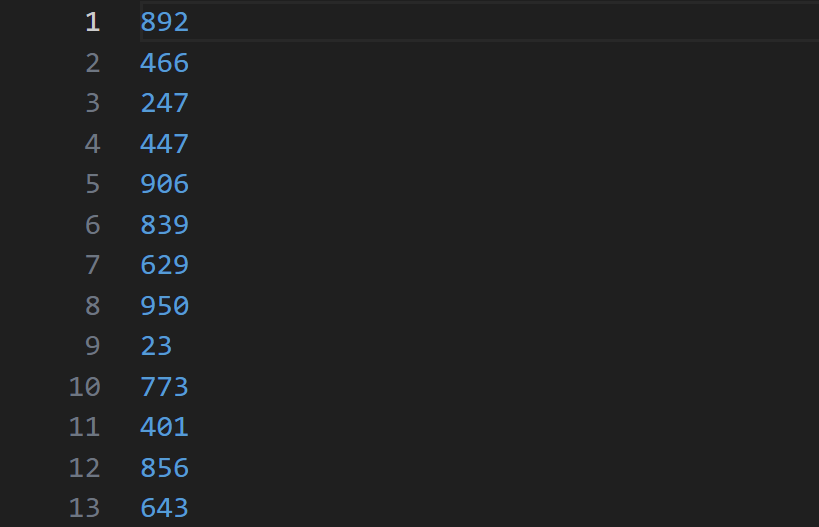
\includegraphics[width=0.8\textwidth]{figures/data.png}
    \caption{数据集示例}
    \label{fig:data} 
\end{figure}

\subsection{最大数据集运行结果截图}
在1,000,000数据集测试下,各个算法的运行结果截图见图\ref{fig:run_reuslt_1}和图\ref{fig:run_reuslt_2}:
\begin{figure}[htbp]
    \centering
    % 第一张子图
    \begin{subfigure}[b]{0.45\textwidth} % 子图宽度为总宽度的45%
        \centering
        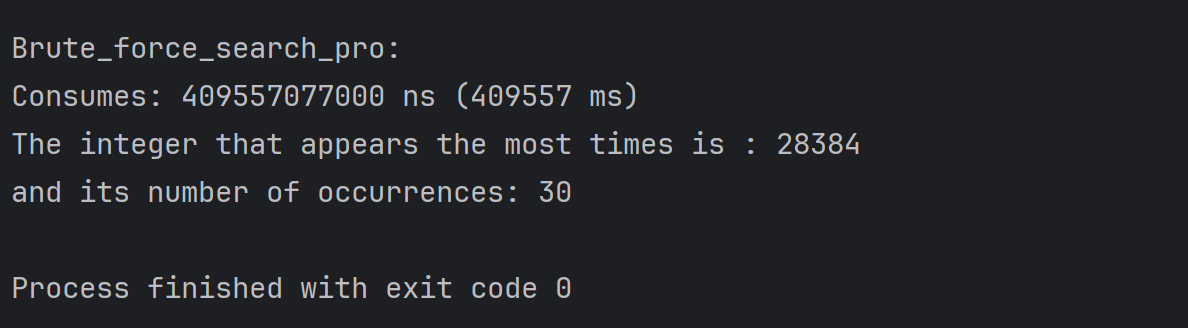
\includegraphics[width=\textwidth]{figures/max_brute_force.png} % 替换为你的图片路径
        \caption{Brute\_Force\_Search\_Pro}
        \label{fig:brute_force_search_pro}
    \end{subfigure}
    \hfill % 添加水平间距
    % 第二张子图
    \begin{subfigure}[b]{0.45\textwidth}
        \centering
        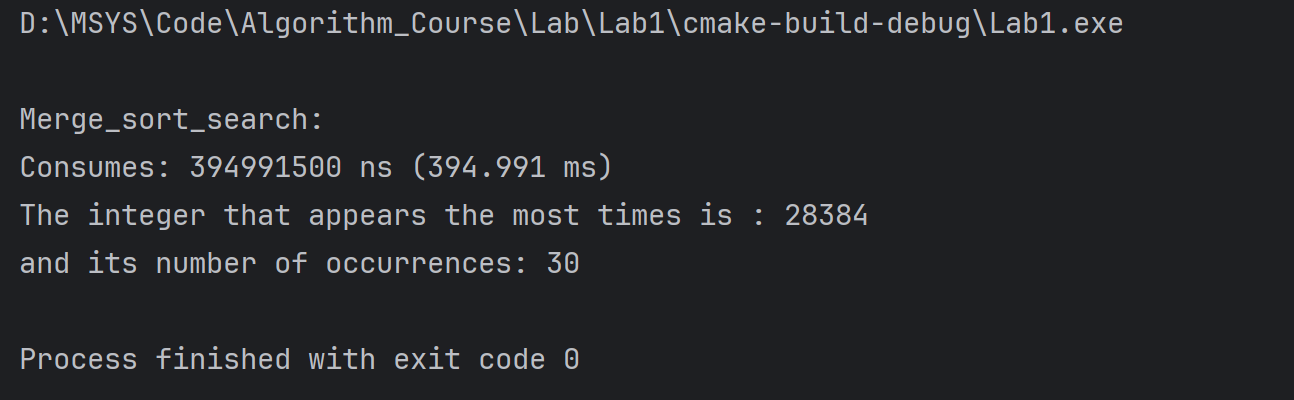
\includegraphics[width=\textwidth]{figures/sort_and_scan.png} % 替换为你的图片路径
        \caption{Sort\_and\_Scan}
        \label{fig:sort_and_scan}
    \end{subfigure}
    % 总图标题
    \caption{lab\_reuslt\_1}
    \label{fig:run_reuslt_1}
\end{figure}

\begin{figure}[htbp]
    \centering
    % 第一张子图
    \begin{subfigure}[b]{0.45\textwidth} % 子图宽度为总宽度的45%
        \centering
        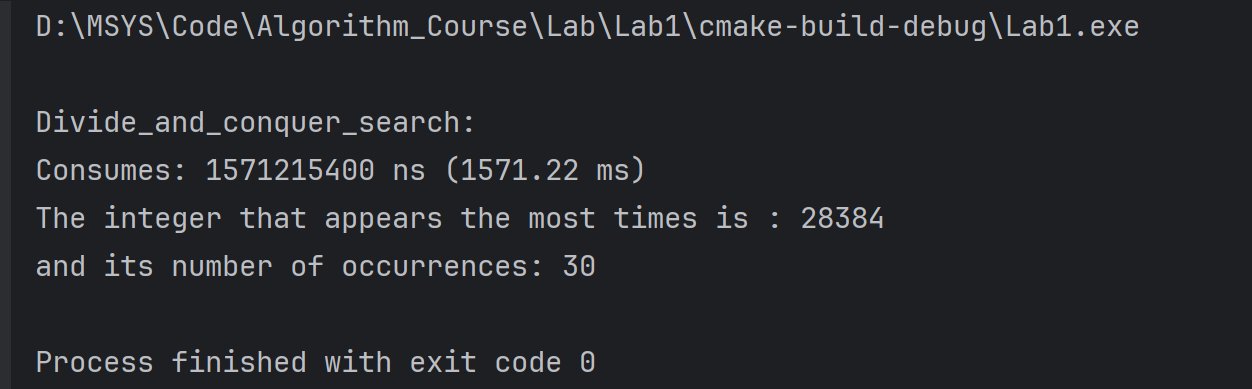
\includegraphics[width=\textwidth]{figures/divide_and_conquer.png} % 替换为你的图片路径
        \caption{Divide\_and\_Conquer}
        \label{fig:divide_and_conquer}
    \end{subfigure}
    \hfill % 添加水平间距
    % 第二张子图
    \begin{subfigure}[b]{0.45\textwidth}
        \centering
        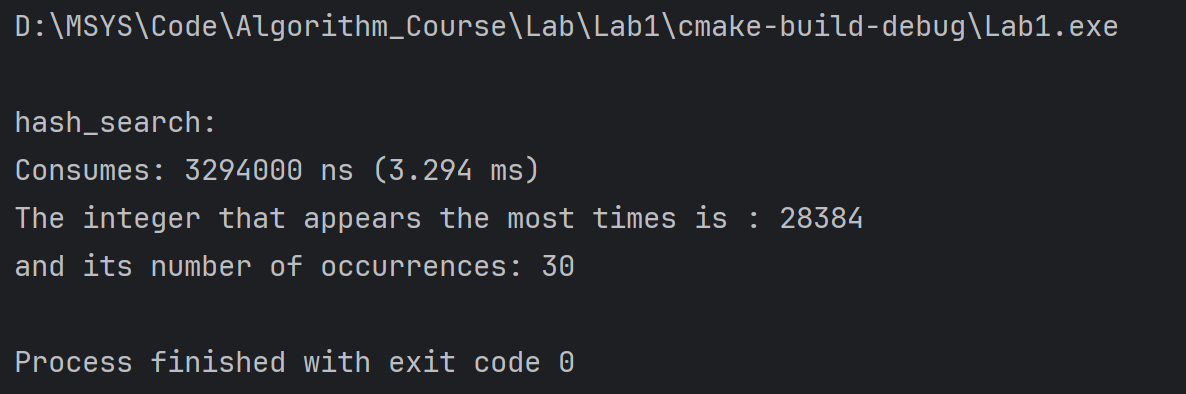
\includegraphics[width=\textwidth]{figures/hash.png} % 替换为你的图片路径
        \caption{Hash}
        \label{fig:hash}
    \end{subfigure}
    % 总图标题
    \caption{lab\_result\_2}
    \label{fig:run_reuslt_2}
\end{figure}

可以发现,四种算法的功能均正确:都找到了出现次数最多的整数:28384,出现次数为:30。
\subsection{实验数据}
实验得到的数据如下:
\begin{table}[h]
    \centering
    \begin{tabular}{|c|c|c|c|c|c|}
    \hline
    数据集规模 & 100 & 1,000 & 10,000 & 100,000 & 1,000,000 \\
    \hline
    暴力搜索改良版 & 0.0253 & 0.5669 & 49.0998 & 4229.89 & 401570\\
    \hline
    先排序后扫描 & 0.0191 & 0.2077 & 2.7056 & 33.5174 & 388.76\\
    \hline
    分治算法 & 0.1649 & 1.0363 & 17.2027 & 138.263 & 1584.6\\
    \hline
    哈希表方法 & 0.0032 & 0.0078 & 0.0563 & 0.3033 & 3.1352\\
    \hline
\end{tabular}
\caption{五种算法在不同规模数据集下的运行时间测试(时间单位: ms)}
\label{tab:time_results}
\end{table}
从表\ref{tab:time_results}可以看出,随着数据规模的增大,各算法的运行时间呈现出明显的差异,这与其理论时间复杂度高度吻合。

\begin{figure}[htbp]
    \centering
    % 第一张子图
    \begin{subfigure}[b]{0.48\textwidth} % 子图宽度为总宽度的45%
        \centering
        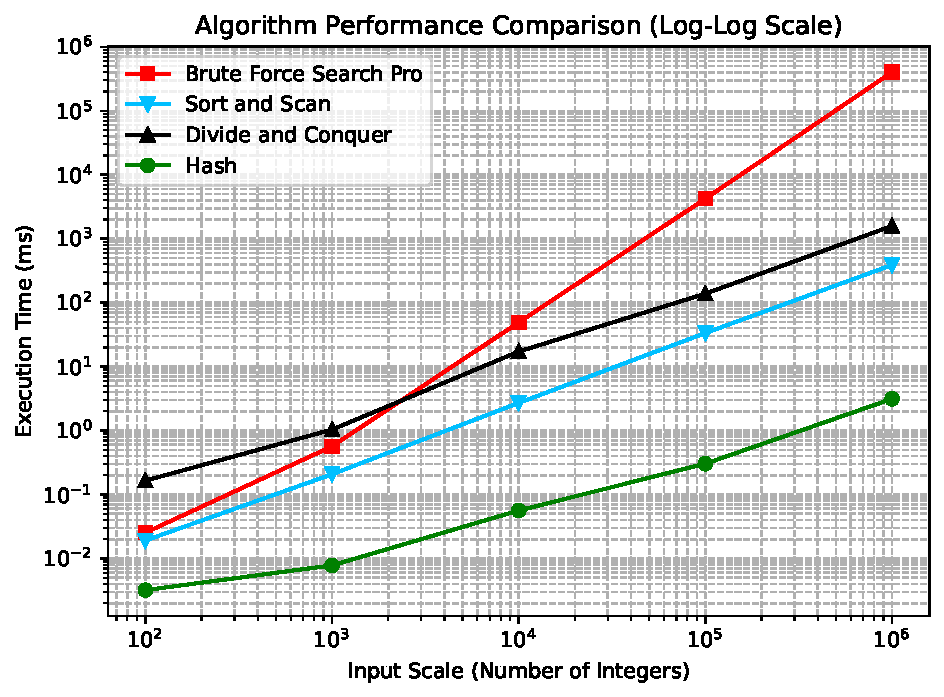
\includegraphics[width=\textwidth]{figures/Time_Scale.pdf} % 替换为你的图片路径
        \caption{Logarithmic coordinates}
        \label{fig:time-scale_log}
    \end{subfigure}
    \hfill % 添加水平间距
    % 第二张子图
    \begin{subfigure}[b]{0.48\textwidth}
        \centering
        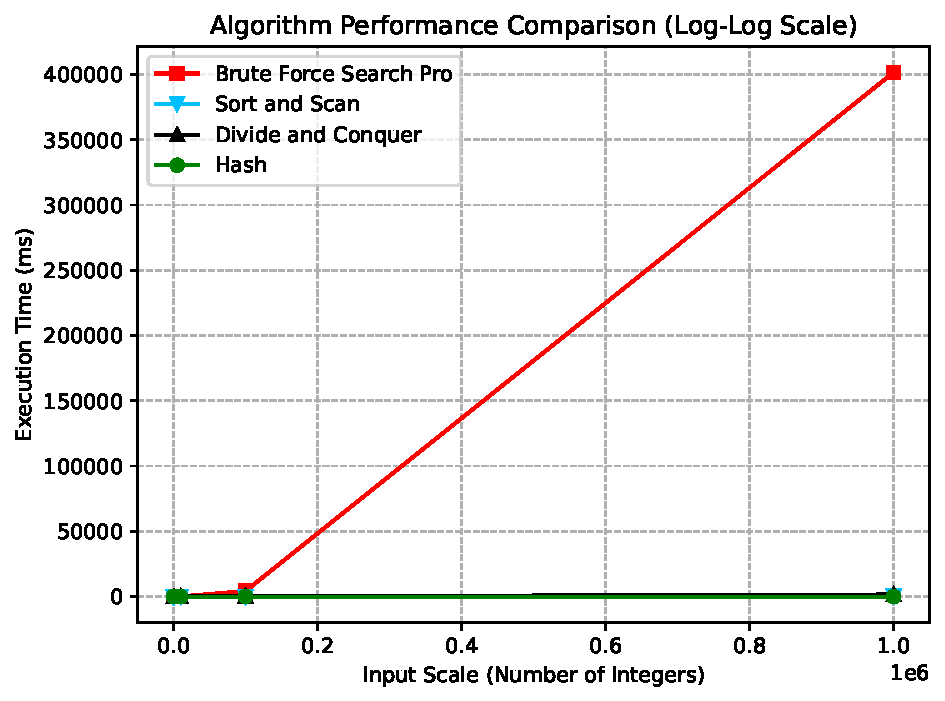
\includegraphics[width=\textwidth]{figures/Time_Scale_Linear.pdf} % 替换为你的图片路径
        \caption{Linear Coordinates}
        \label{fig:time-scale_lin}
    \end{subfigure}
    % 总图标题
    \caption{execution time - input scales curve}
    \label{fig:time-scale}
\end{figure}
图\ref{fig:time-scale}直观地展示了各算法随数据规模增长的时间复杂度特性。在对数坐标系中,曲线斜率反映了算法的时间复杂度级别。斜率越大,代表增长的越剧烈。在图\ref{fig:time-scale_lin}中更加明显地反映了这一点。
% --------------------------------------------------------------------------------------------------------
\newpage
\section{分析与讨论}

\subsection{结果分析}
基于表\ref{tab:time_results}和图\ref{fig:time-scale}所示的实验结果,可以得出以下重要结论:

\paragraph{时间复杂度验证}
各算法的实际运行时间表现与其理论时间复杂度高度一致:
\begin{itemize}
    \item \textbf{暴力搜索算法}:在小数据量(100-1,000)下尚可接受,但在10,000数据量时耗时49.09ms,100,000时急剧上升至4229ms,呈$O(n^2)$增长趋势,验证了其平方级时间复杂度。
    \item \textbf{先排序后扫描算法}:在100,000数据量下仅需33.52ms,相比暴力搜索有超过100倍的性能提升,体现了$O(n\log n)$算法的优势。
    \item \textbf{分治算法}:表现稳定,在100,000数据量下耗时138.26ms,虽然略慢于排序算法,但仍保持了$O(n\log n)$的良好性能。
    \item \textbf{哈希表方法}:表现最为优异,在100,000数据量下仅需0.30ms,1,000,000数据量也只需3.13ms,完美体现了$O(n)$线性时间复杂度的优势。
\end{itemize}

\paragraph{算法改进空间}
\begin{itemize}
    \item 暴力搜索算法几乎没有改进空间,其高时间复杂度本质决定了不适用于大规模数据
    \item 排序算法可尝试使用快速排序等原地排序算法来减少空间开销。本算法虽然采用了辅助数组辅助排序,减少了递归函数中对栈空间的大量占用,但是仍可进一步优化。
    \item 哈希表方法在数据范围较大时可考虑使用真正的哈希表来节省空间
\end{itemize}

\subsection{实验后的思考}

本次实验让我深刻体会到算法理论分析与实际性能的高度一致性。在课堂中,$O(n^2)$、$O(n\log n)$、$O(n)$等复杂度概念相对抽象,但通过编写程序、测试不同规模数据集后,这些概念变得非常直观。特别是观察到暴力搜索算法在数据量达到1,000,000时运行时间超过6min,而哈希表方法仅需3 ms,这种数量级的差异让我对算法复杂度有了更深刻的认识。

此外,作为本次实验的重点,分治算法的实现让我理解了"分而治之"思想在实际问题中的应用。虽然分治算法在性能上不如专门的哈希表方法,但其设计思路具有重要的理论价值。特别是在处理无法直接建立映射表的数据类型时,分治算法提供了一种更加通用的解决方案。


% 参考文献如不需要,将如下两行注释掉
% \bibliographystyle{plain}
% \bibliography{./template}  %bib文件名

\end{document}
